Dopo aver verificato separatamente i singoli componenti metodologici, il presente capitolo considera la pipeline GDM nella sua configurazione completa mediante un esperimento dinamico end-to-end. L'obiettivo è valutare il comportamento del framework quando il mesh mover neurale, il \textit{Safety Filter}, il solutore FEM e il meccanismo di evoluzione o trasferimento della mesh operano congiuntamente durante l'integrazione temporale della PDE.

Il confronto finale è organizzato attorno a tre aspetti distinti ma strettamente correlati: accuratezza della soluzione numerica, costo computazionale complessivo e robustezza geometrica della discretizzazione. In particolare, viene confrontato il riferimento a mesh fissa con differenti strategie di gestione della mesh mobile basate sul medesimo modello GNN: il remapping pointwise $P_1$, la proiezione $L^2$ e la formulazione ALE continua. L'obiettivo non è stabilire una superiorità assoluta di una singola configurazione, ma quantificare il compromesso tra accuratezza, costo e gestione della mesh associato ai differenti meccanismi di accoppiamento.

\subsection{Configurazione del benchmark e baseline di confronto}

\label{subsec:benchmark_setup}

La campagna di valutazione dinamica end-to-end adotta la configurazione fisica di convezione--diffusione e la Manufactured Solution analitica $u^\star(\mathbf{x},t)$ definite nella Sezione~\ref{subsec:pde_governing}, operando sul dominio $\Omega=[0,1]^2$ fino all'istante finale $T=0.5$, con

\[
\mathbf{b}=(0.4,0.2)^T,
\qquad
\nu=10^{-3}.
\]

La triangolazione di partenza è uniforme a risoluzione $32\times32$, corrispondente a $N=1089$ nodi e $M=2048$ elementi triangolari $P_1$. L'integrazione temporale utilizza lo schema Backward Euler con passo costante

\[
\Delta t=5\times10^{-3},
\]

su un totale di $100$ passi temporali. L'aggiornamento della configurazione geometrica viene effettuato ogni $N_a=10$ passi.

A ciascun evento di adattamento, la MeshMover GNN riceve lo stato FEM disponibile durante la simulazione e produce uno spostamento nodale. Lo spostamento viene quindi sottoposto al Deterministic Safety Filter, introdotto nella Sezione~\ref{subsec:safety_filter}, che verifica l'ammissibilità della traiettoria lineare della mesh rispetto alla soglia

\[
\epsilon=10^{-4}.
\]

Tale controllo è applicato secondo le ipotesi geometriche definite nel Capitolo~\ref{sec:gdm_framework} e non viene interpretato come una proprietà generale indipendente dalla discretizzazione considerata.

Per il benchmark finale vengono confrontate quattro configurazioni:

\begin{table}[htbp]
\centering
\small
\setlength{\tabcolsep}{3pt}
\caption{Configurazioni considerate nel benchmark dinamico finale.}
\label{tab:final_baselines}
\begin{tabular*}{\linewidth}{@{\extracolsep{\fill}}lcccc@{}}
\toprule
Configurazione &
\begin{tabular}[c]{@{}c@{}}Mesh\\ mobile\end{tabular} &
GNN &
\begin{tabular}[c]{@{}c@{}}Trasferimento\\ dello stato\end{tabular} &
ALE \\
\midrule
Fixed FEM   & No  & No  & --                & No \\
GDM + $P_1$ & Sì  & Sì  & $P_1$ pointwise   & No \\
GDM + $L^2$ & Sì  & Sì  & Proiezione $L^2$  & No \\
GDM + ALE   & Sì  & Sì  & Nessuno           & Sì \\
\bottomrule
\end{tabular*}
\end{table}

La configurazione \textit{Fixed FEM} costituisce il riferimento Euleriano e permette di quantificare l'errore ottenuto senza alcun movimento della mesh. La configurazione \textit{GDM + $P_1$} rappresenta l'accoppiamento con il remapping pointwise barycentrico, già analizzato nelle prove dello Stage B. La configurazione \textit{GDM + $L^2$} sostituisce il trasferimento pointwise con la proiezione globale introdotta nella Sezione~\ref{subsec:l2_projection}. Infine, \textit{GDM + ALE} elimina il trasferimento esplicito dello stato e incorpora il moto della mesh direttamente nella formulazione della PDE attraverso la velocità relativa.

Il modello neurale impiegato è identico per tutte le configurazioni basate sulla GNN e corrisponde al checkpoint addestrato offline nello Stage A, senza fine-tuning specifico per il problema transiente.

Per rendere il confronto tra $L^2$ e ALE il più possibile controllato, viene utilizzata la medesima sequenza temporale di configurazioni geometriche target prodotte dalla GNN. Questo protocollo deve tuttavia essere distinto dalla traiettoria calcolata direttamente durante la campagna dinamica dello Stage B: i target vengono prescritti agli istanti di adattamento e successivamente riutilizzati nel confronto finale. Nel caso $L^2$, la mesh viene portata direttamente alla configurazione target e lo stato viene trasferito mediante proiezione; nel caso ALE, lo stesso spostamento viene distribuito sui successivi $N_a$ passi e trasformato nella velocità di mesh

\[
\mathbf{w}
=
\frac{\Delta\mathbf{X}_{\mathrm{safe}}}
{N_a\Delta t}.
\]

La differenza tra i due protocolli è quindi intenzionale e consente di confrontare principalmente il meccanismo di gestione del moto della mesh, senza introdurre variazioni nel modello neurale o nella sequenza dei target geometrici.

È inoltre importante notare che i valori ottenuti in questo benchmark finale non coincidono necessariamente con quelli riportati nella diagnostica dinamica dello Stage B. In particolare, il protocollo di replay dei target geometrici adottato nel presente capitolo non coincide punto per punto con la traiettoria numerica generata nel corso della precedente campagna dinamica; i risultati devono pertanto essere confrontati all'interno del rispettivo protocollo sperimentale.

\subsection{Accuratezza della PDE ed evoluzione temporale dell'errore}

\label{subsec:error_dynamics}

La prima metrica considerata è l'errore relativo in norma $L^2$ rispetto alla soluzione manufactured,

\begin{equation}
E_{L^2}(t)
=
\frac{
\|u_h(\cdot,t)-u_{\mathrm{exact}}(\cdot,t)\|_{L^2(\Omega)}
}{
\|u_{\mathrm{exact}}(\cdot,t)\|_{L^2(\Omega)}
},
\label{eq:final_l2_error}
\end{equation}

calcolato a ogni passo temporale. Oltre al valore finale $E_{L^2}(T)$, viene considerato l'errore integrato nel tempo,

\begin{equation}
\overline{E}_{L^2}
=
\frac{1}{T}
\int_0^T
E_{L^2}(t)\,dt,
\label{eq:final_integrated_error}
\end{equation}

approssimato numericamente sulla griglia temporale del benchmark.

Il valore finale misura la precisione raggiunta al termine della simulazione, mentre l'errore integrato nel tempo sintetizza il comportamento complessivo della soluzione e permette di evidenziare eventuali perturbazioni associate agli eventi di adattamento.

\begin{table}[htbp]
\centering
\caption{Accuratezza globale nel benchmark dinamico finale. I valori sono espressi come percentuale dell'errore relativo $L^2$.}
\label{tab:final_accuracy}
\begin{tabular}{lcc}
\toprule
Configurazione
& $E_{L^2}(T)$ [\%]
& $\overline{E}_{L^2}$ [\%]
\\
\midrule
Fixed FEM
& 9.03
& 7.96
\\
GDM + $P_1$
& 12.72
& 10.32
\\
GDM + $L^2$
& 8.92
& 7.87
\\
GDM + ALE
& 9.47
& 8.27
\\
\bottomrule
\end{tabular}
\end{table}

Il confronto mostra innanzitutto una differenza netta tra i due meccanismi di trasferimento esplicito considerati. La configurazione GDM + $P_1$ raggiunge un errore finale del $12.72\%$ e un errore integrato del $10.32\%$, superiori ai corrispondenti valori della mesh fissa. Il risultato è coerente con la diagnostica dello Stage B, nella quale l'applicazione reiterata del remapping pointwise aveva evidenziato un accumulo dell'errore di trasferimento.

La sostituzione del remapping pointwise con la proiezione $L^2$ porta invece a un errore finale dell'$8.92\%$ e a un errore integrato del $7.87\%$. Nel protocollo considerato, questi valori risultano molto vicini a quelli della mesh fissa, con una differenza rispettivamente di circa $0.11$ e $0.09$ punti percentuali. Il risultato indica che la proiezione globale riduce il contributo del trasferimento osservato con il remapping pointwise, senza tuttavia implicare che il movimento della mesh renda in generale la discretizzazione più accurata della baseline fissa.

La formulazione GDM + ALE raggiunge invece un errore finale del $9.47\%$ e un errore integrato dell'$8.27\%$. Rispetto alla proiezione $L^2$, lo scostamento è pari a circa $0.55$ punti percentuali sul valore finale e $0.40$ punti percentuali sul valore integrato. In questo benchmark, quindi, la formulazione ALE conserva un livello di accuratezza comparabile ma leggermente inferiore a quello ottenuto con la proiezione $L^2$.

L'evoluzione temporale dell'errore riportata in Figura~\ref{fig:final_error_dynamics} permette di osservare ulteriormente la differenza tra le strategie di accoppiamento.

\begin{figure}[htbp]
\centering
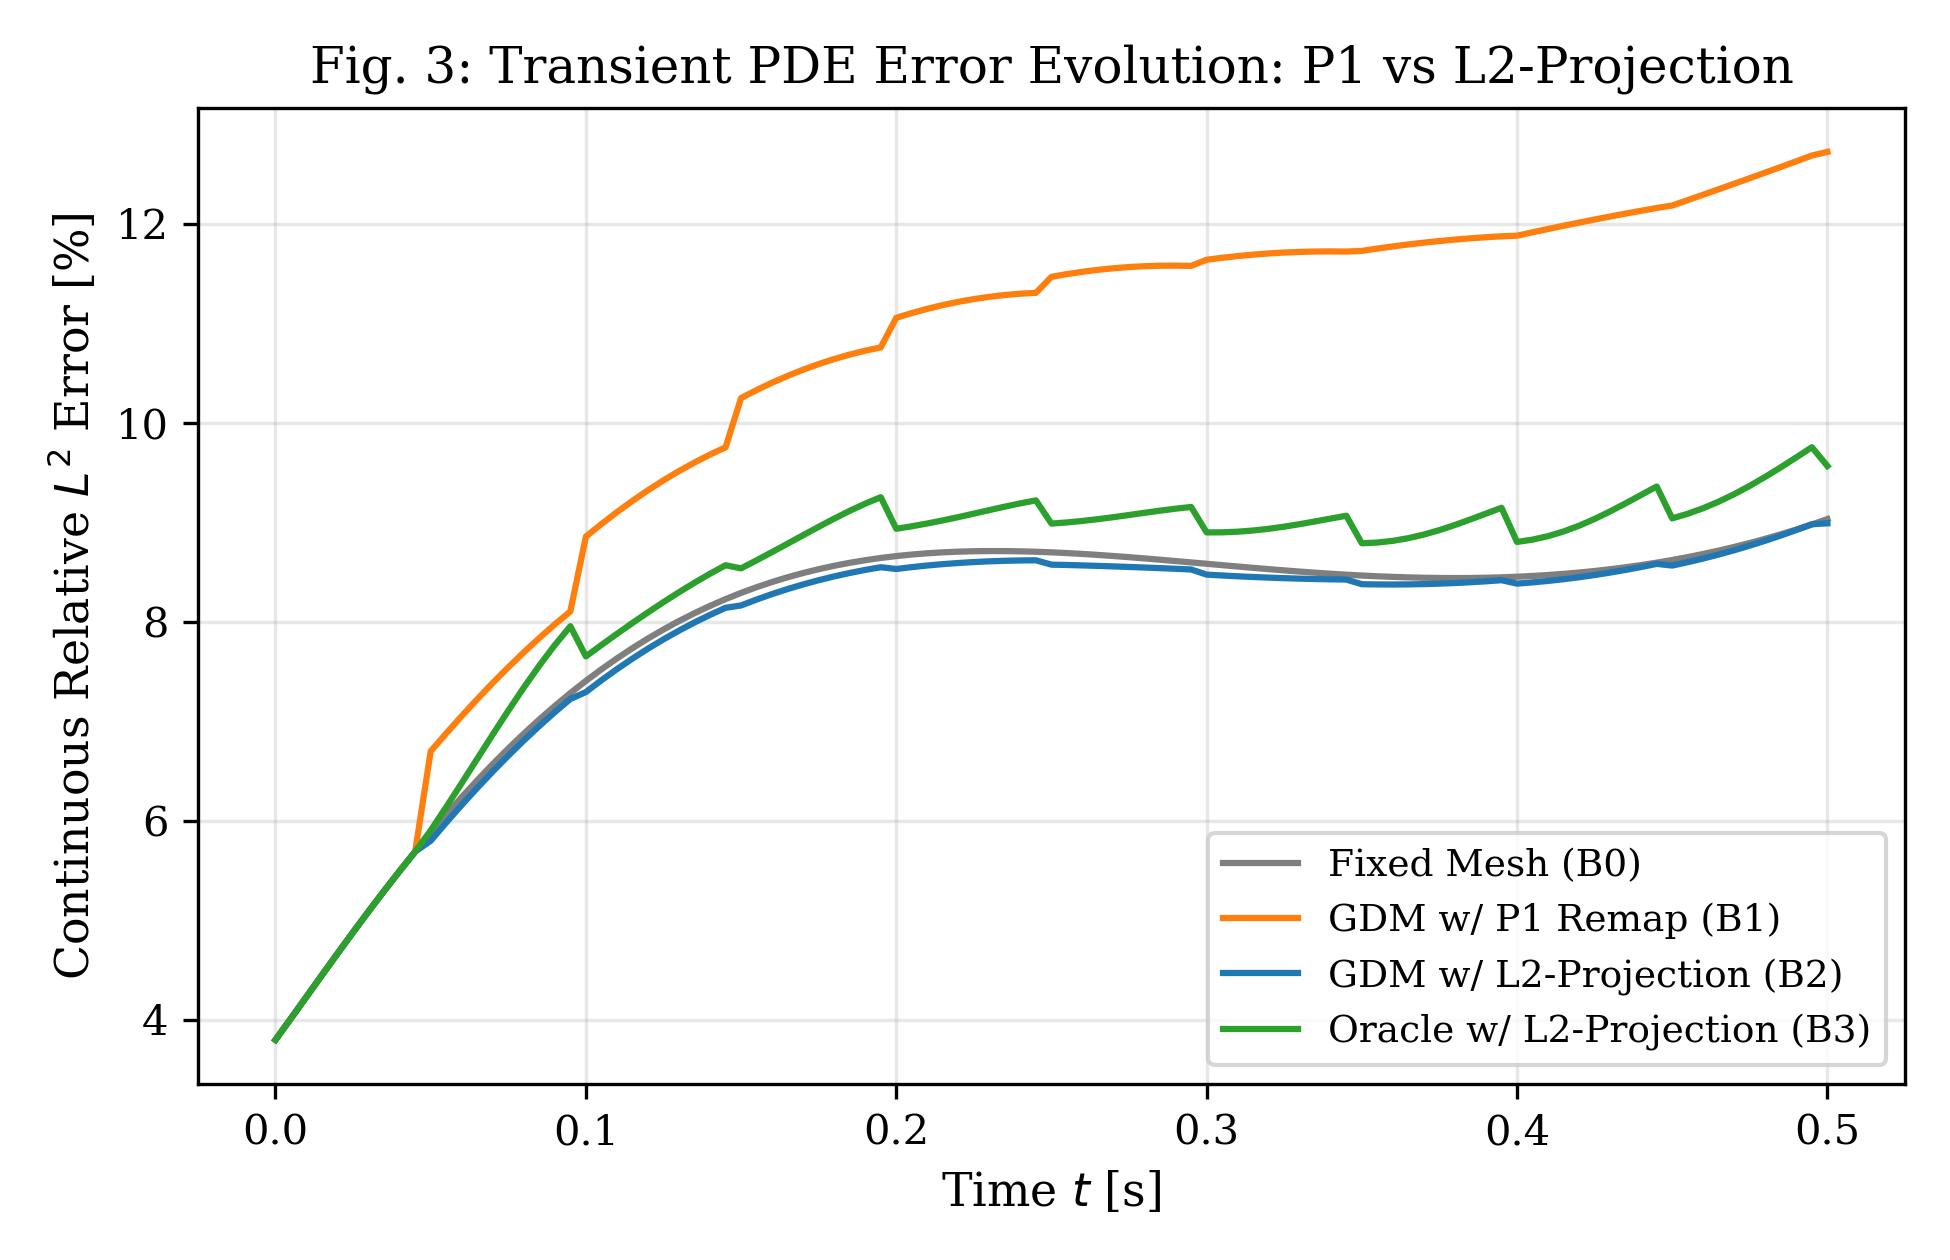
\includegraphics[width=0.92\linewidth]{images/stage_b/fig3_dynamic_pde_error.png}
\caption{Evoluzione temporale dell'errore relativo $L^2$ nelle configurazioni dinamiche considerate.}
\label{fig:final_error_dynamics}
\end{figure}

La curva associata al remapping $P_1$ evidenzia una crescita dell'errore compatibile con l'accumulo del contributo introdotto dai trasferimenti successivi. Nel caso della proiezione $L^2$, l'errore rimane invece più vicino a quello della mesh fissa, sebbene siano osservabili variazioni localizzate in corrispondenza degli eventi di trasferimento.

La formulazione ALE presenta un'evoluzione temporale più regolare, poiché il cambiamento geometrico viene distribuito nel tempo e non richiede una fase separata di riproiezione dello stato. Il prezzo di tale continuità è, nel benchmark considerato, un errore leggermente superiore alla configurazione con proiezione $L^2$.

Nel complesso, il confronto conferma che la scelta del meccanismo di accoppiamento tra mesh mobile e stato fisico costituisce una componente determinante del comportamento end-to-end. La qualità della geometria prodotta dalla GNN non è quindi sufficiente, da sola, a caratterizzare la precisione della simulazione.

\subsection{Costo computazionale e scomposizione del runtime}

\label{subsec:runtime_analysis}

L'accuratezza viene valutata congiuntamente al costo computazionale introdotto dall'adattamento. Il tempo totale di simulazione può essere scomposto concettualmente come

\begin{equation}
T_{\mathrm{total}}
=
T_{\mathrm{FEM}}
+
T_{\mathrm{GNN}}
+
T_{\mathrm{Safety}}
+
T_{\mathrm{Remap}}
+
T_{\mathrm{other}},
\label{eq:runtime_decomposition}
\end{equation}

dove $T_{\mathrm{FEM}}$ rappresenta il costo associato all'assemblaggio e alla soluzione del sistema FEM, $T_{\mathrm{GNN}}$ il costo di inferenza del mesh mover, $T_{\mathrm{Safety}}$ il costo del filtro geometrico e $T_{\mathrm{Remap}}$ il costo dell'eventuale trasferimento esplicito dello stato.

Per la formulazione ALE, il termine $T_{\mathrm{Remap}}$ è assente dalla pipeline, poiché lo stato non viene proiettato esplicitamente tra due configurazioni successive. Restano naturalmente i costi associati all'aggiornamento della geometria, al calcolo della velocità di mesh e alla costruzione degli operatori FEM sulla configurazione corrente.

Nel benchmark transiente unificato a $100$ passi temporali, la configurazione GDM + $L^2$ registra un tempo di esecuzione totale pari a

\begin{equation}
\begin{aligned}
T_{\mathrm{total}}^{L^2}
&=
4.18\ \mathrm{s},
\\
T_{\mathrm{Remap}}^{L^2}
&=
3.35\ \mathrm{s},
\end{aligned}
\label{eq:runtime_l2}
\end{equation}

con il trasferimento dello stato che rappresenta circa l'$80.1\%$ del tempo totale della pipeline in questo benchmark.

La formulazione GDM + ALE completa invece la simulazione in

\begin{equation}
T_{\mathrm{total}}^{\mathrm{ALE}}
=
1.76\ \mathrm{s},
\qquad
T_{\mathrm{Remap}}^{\mathrm{ALE}}
\equiv 0.
\label{eq:runtime_ale}
\end{equation}

Il rapporto tra i tempi complessivi definisce lo speedup operativo della formulazione ALE rispetto alla configurazione con proiezione $L^2$:

\begin{equation}
S_{\mathrm{ALE}}
=
\frac{
T_{\mathrm{total}}^{L^2}
}{
T_{\mathrm{total}}^{\mathrm{ALE}}
}
=
\frac{4.18\ \mathrm{s}}{1.76\ \mathrm{s}}
\approx
2.37\times.
\label{eq:ale_speedup}
\end{equation}

\begin{figure}[htbp]
\centering
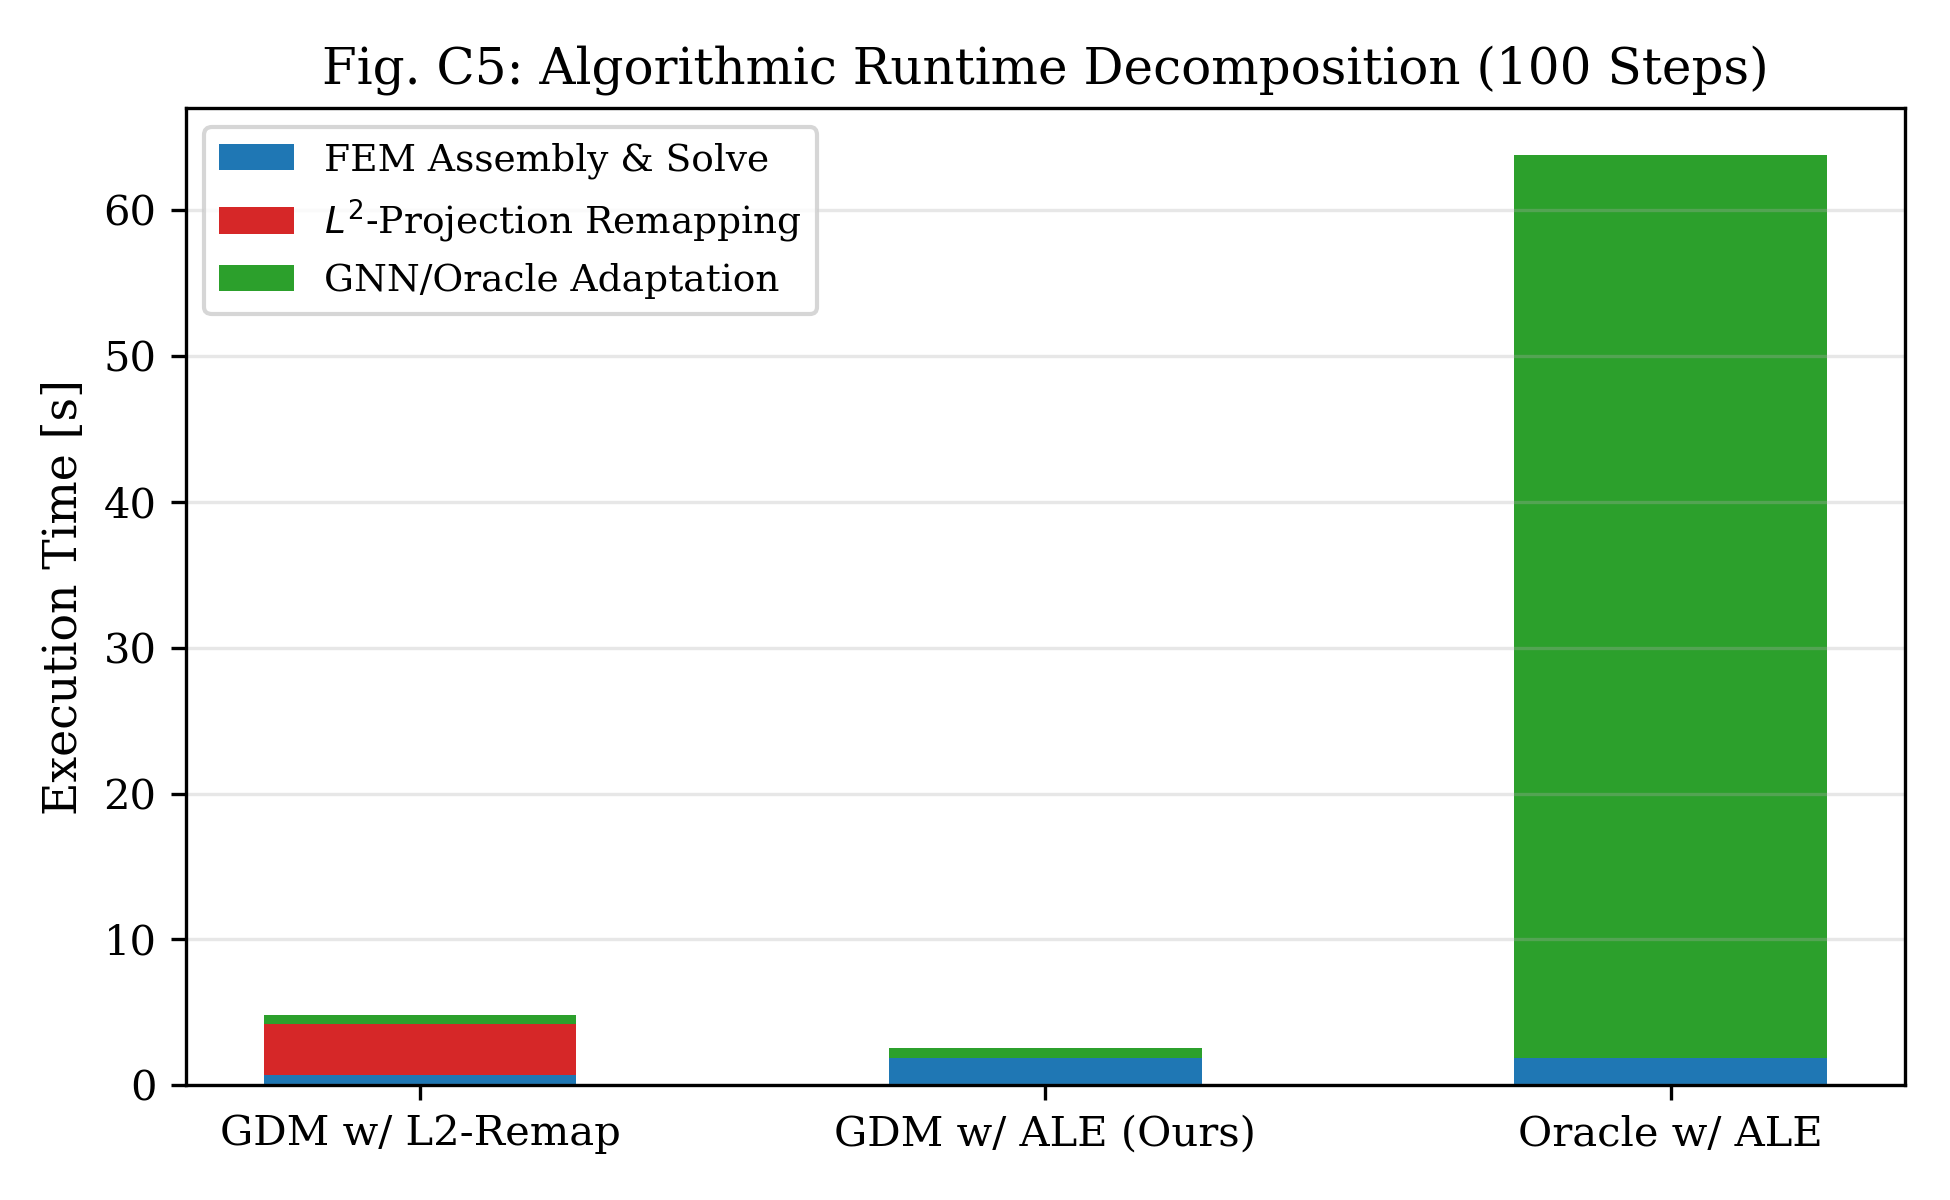
\includegraphics[width=0.90\linewidth]{images/stage_c/fig_c5_runtime_decomposition.png}
\caption{Confronto del costo computazionale tra la strategia con proiezione $L^2$ e la formulazione ALE. Il benchmark mostra uno speedup complessivo di $2.37\times$ per la configurazione ALE.}
\label{fig:final_runtime}
\end{figure}

Il risultato evidenzia che, nel caso considerato, il costo della proiezione dello stato costituisce la componente dominante della pipeline con remapping $L^2$. La formulazione ALE elimina tale operazione separata e riduce il tempo complessivo di simulazione da $4.18$ s a $1.76$ s.

Lo speedup osservato deve tuttavia essere interpretato come un risultato sperimentale specifico del benchmark e non come una stima asintotica generale della convenienza dell'ALE. Esso dipende infatti dalla frequenza di adattamento, dal costo della proiezione, dalla dimensione della discretizzazione e dall'implementazione del solutore.

\subsection{Robustezza geometrica e tracking dinamico della mesh}

\label{subsec:geometric_robustness}

La validazione conclusiva riguarda la qualità geometrica della triangolazione lungo l'intera sequenza temporale. A differenza dello stress test isolato condotto nello Stage A, nel quale la rete veniva volutamente sottoposta a spostamenti amplificati, in questa sezione viene considerato il regime nominale della simulazione dinamica.

Durante l'intera simulazione di $100$ passi temporali, utilizzando il gradiente FEM ricostruito a runtime, il minimo determinante Jacobiano orientato osservato su tutti gli elementi è

\begin{equation}
\min_{t\in(0,T]}
\min_{e=1,\ldots,M}
J_e(t)
\approx
6.59\times10^{-4}
>
\epsilon,
\label{eq:final_min_j}
\end{equation}

con $\epsilon=10^{-4}$. Il valore iniziale della mesh indeformata è

\[
J_0=9.77\times10^{-4}.
\]

Nel benchmark nominale il fattore globale del Safety Filter rimane

\[
\alpha_{\mathrm{global}}(t)=1
\]

per tutte le finestre di adattamento. Ciò significa che le configurazioni previste dalla GNN risultano già ammissibili rispetto alla soglia geometrica e che il filtro non deve ridurre gli spostamenti.

Questo risultato deve essere distinto dalla funzione di protezione verificata nello stress test dello Stage A: in quel caso il filtro veniva attivato intenzionalmente mediante amplificazione dello spostamento, mentre nel benchmark nominale non è stato necessario alcun intervento correttivo.

\begin{figure}[htbp]
\centering
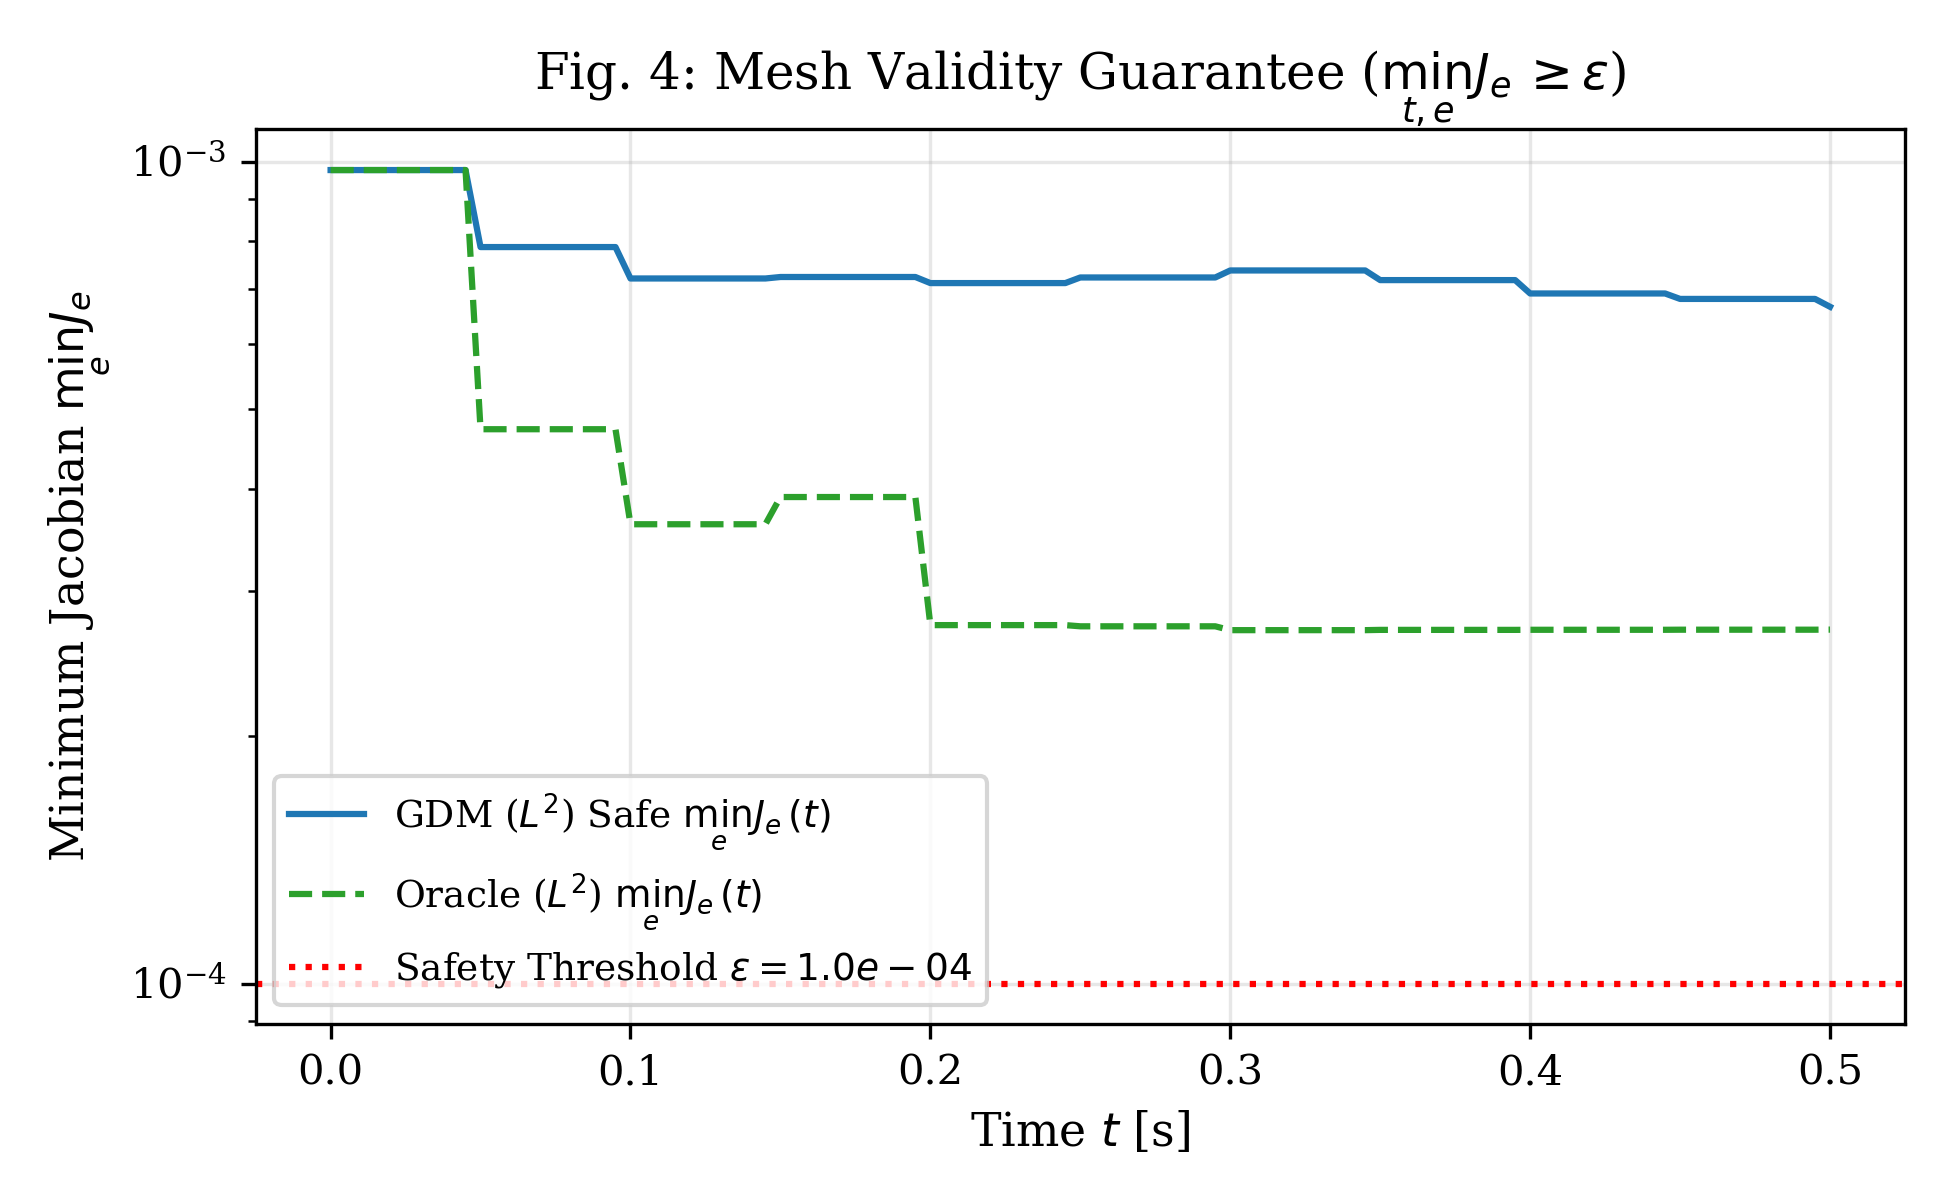
\includegraphics[width=0.92\linewidth]{images/stage_b/fig4_mesh_safety_over_time.png}
\caption{Evoluzione temporale del minimo determinante orientato $J_{\min}(t)$ durante la simulazione dinamica. La linea orizzontale rappresenta la soglia geometrica $\epsilon$.}
\label{fig:final_mesh_safety}
\end{figure}

L'analisi di $J_{\min}(t)$ deve essere interpretata insieme all'evoluzione di $\alpha_{\mathrm{global}}(t)$ e agli istanti di adattamento. Un valore $\alpha_{\mathrm{global}}=1$ indica che la configurazione proposta è direttamente ammissibile; un valore inferiore a uno segnalerebbe invece l'attivazione del filtro e la conseguente contrazione dello spostamento.

La proprietà osservata riguarda esclusivamente la validità geometrica della discretizzazione e non costituisce, di per sé, una proprietà di conservazione della soluzione PDE. La consistenza geometrica e il comportamento del trasferimento dello stato sono stati verificati separatamente nel Capitolo~\ref{sec:diagnostics} mediante i test di Stage B e Stage C.

\begin{figure}[htbp]
\centering
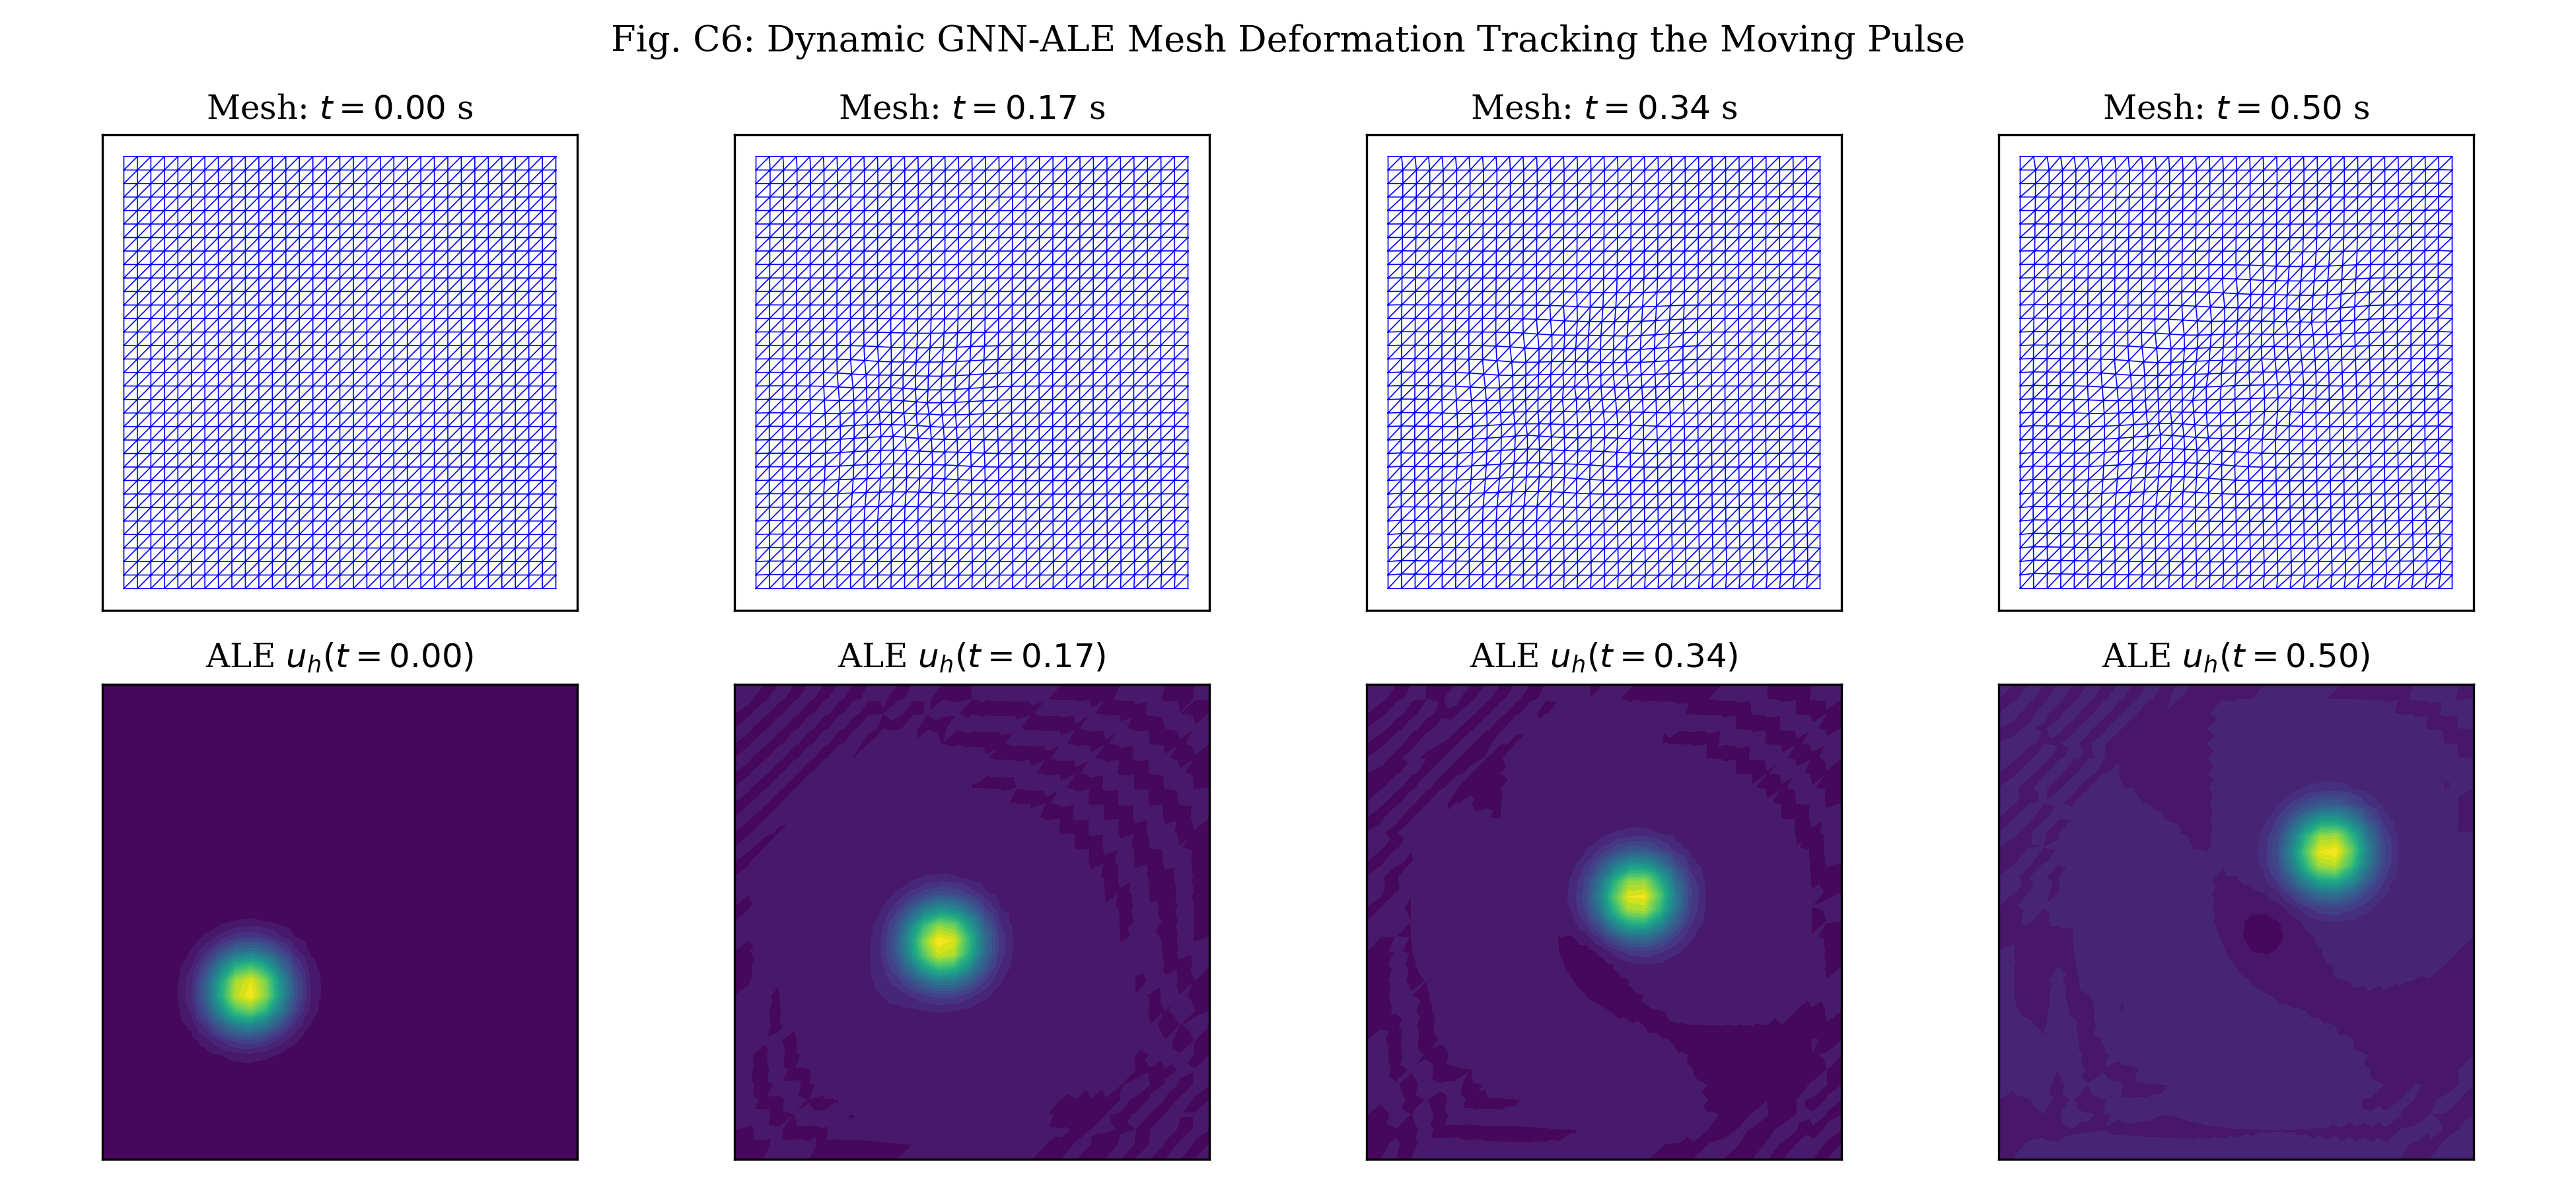
\includegraphics[width=0.90\linewidth]{images/stage_c/fig_c6_qualitative_tracking.png}
\caption{Esempio qualitativo del tracking della struttura della soluzione durante l'evoluzione dinamica con mesh adattata.}
\label{fig:final_tracking}
\end{figure}

Nel complesso, il benchmark dinamico mostra che l'integrazione della GNN con il controllo geometrico deterministico mantiene una triangolazione ammissibile durante l'intera simulazione considerata. Nel regime nominale analizzato, il Safety Filter non altera la traiettoria predetta dalla GNN; il principale effetto della scelta tra remapping $L^2$ e formulazione ALE riguarda quindi il trattamento dello stato fisico e il conseguente compromesso tra accuratezza e costo computazionale.
